\chapter{Trabalhos Futuros}
\label{c:trabalhos_futuros}

Durante o desenvolvimento do sistema proposto inicialmente, surgiram algumas possibilidades de melhorias futuras para o projeto, de maneira a abranger maiores necessidades na pesquisa por soluções econômicas em relação ao consumo energético da Universidade Federal de Goiás.

\section{Melhoramento da Coleta de Dados}

Uma melhor maneira de acesso aos dados dos medidores irá ocasionar na coleta de maiores variáveis de medição, possibilitando assim melhores análises desses dados. Atualmente a API do sistema da CCK disponibiliza apenas a coleta dos dados de potência, enquanto que os dados de tensão, corrente, fator de potência, entre outros, são visíveis apenas no sistema proprietário da empresa. Com uma abertura desse sistema, ou até mesmo o desenvolvimento de outro modo de obtenção dos dados dos medidores, essa limitação seria vencida.

Outra alternativa seria o uso de outro dispositivo, ou até mesmo o desenvolvimento de um dispositivo próprio da Universidade. Porém esta é uma alternativa que ocasiona um custo mais elevado em comparação com uma nova solução de software.

\section{Melhoramento da Estrutura de Dados}

O desenvolvimento da estrutura de dados foi menor devido ao escopo do projeto, porém esta estrutura pode abranger outras entidades, como por exemplo inventário de equipamentos, bem como as entidades existentes podem ser expandidas com outras informações, por exemplo número de patrimônio endereço IP, entre outras.

Essas modificações, ao serem aplicadas no banco podem ser acessadas por qualquer sistema que faça uso do mesmo, uma vez que o banco de dados será a estrutura central de armazenamento das informações da rede de medição da Universidade. 

\newpage

\section{Desenvolvimento de Aplicação Mobile para acesso aos dados}

Apesar do SIDE ser uma aplicação web responsiva, o desenvolvimento de uma aplicação \textit{mobile} tornaria a experiência de consumo dos dados muito mais adequada à realidade atual, uma vez que o uso de dispositivos móveis é basicamente uma unanimidade visto que o Brasil é hoje o quinto país no uso de dispositivos móveis\footnote{\textit{The State of Mobile in 2019}: \url{https://www.appannie.com/en/insights/market-data/the-state-of-mobile-2019/}}.

\begin{figure}[H]
    \centering
    \caption{Exemplo Tela Responsiva SIDE}
    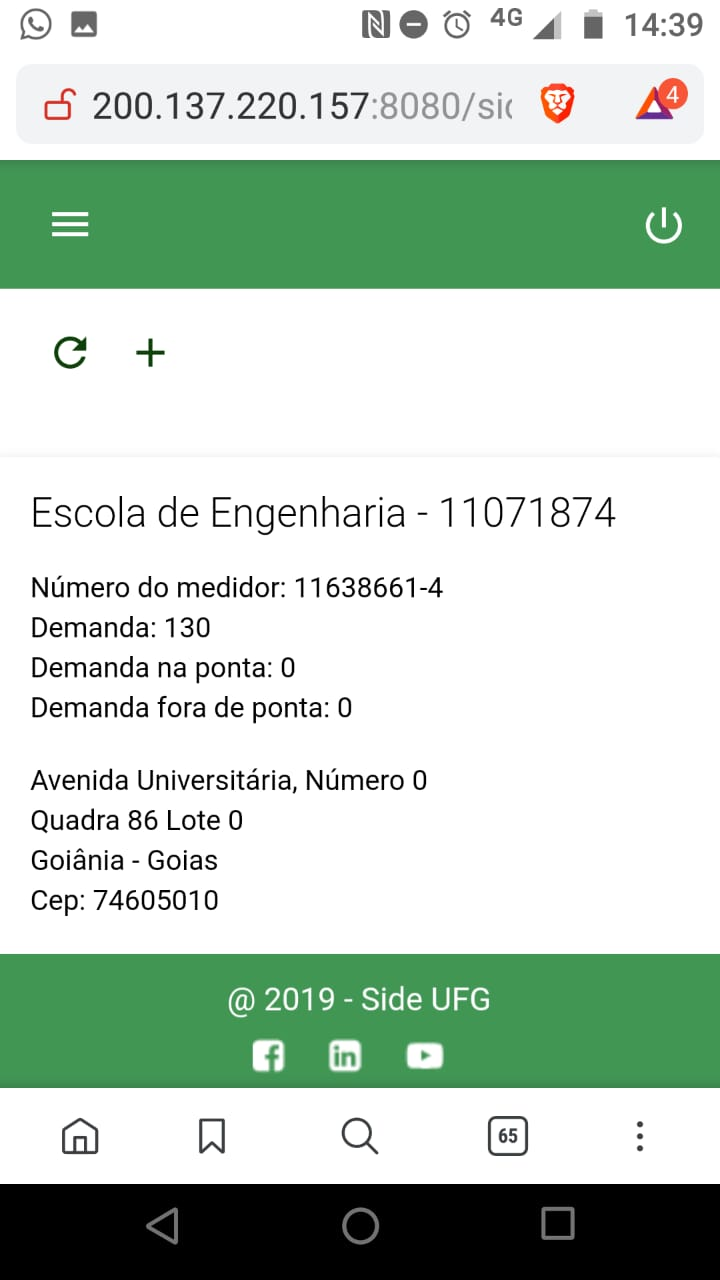
\includegraphics[width=0.5\linewidth]{imagens/side/side-web-01.jpeg}
    \caption*{Fonte: Próprio Autor}
    \label{fig:mobile-01}
\end{figure}

\begin{figure}[H]
    \centering
    \caption{Menu Mobile SIDE}
    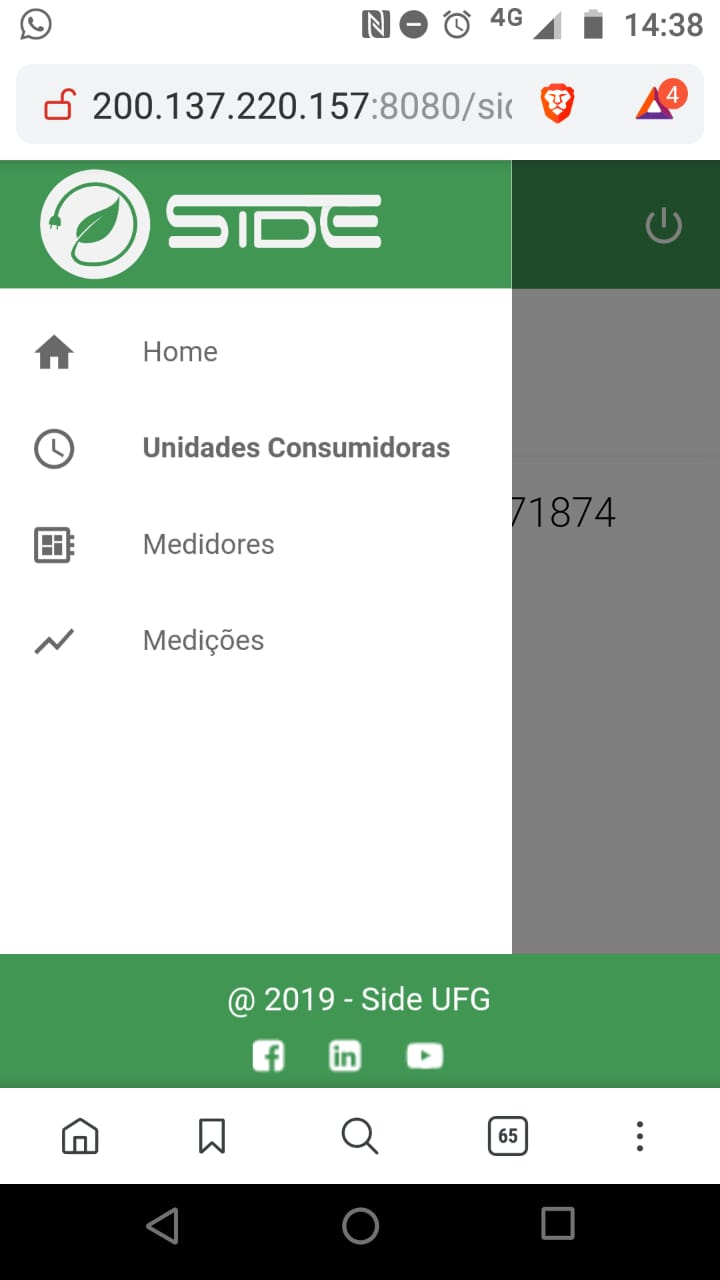
\includegraphics[width=0.5\linewidth]{imagens/side/side-web-02.jpeg}
    \caption*{Fonte: Próprio Autor}
    \label{fig:mobile-02}
\end{figure}

Devido ao uso de um \textit{framework} de desenvolvimento, a parte de modelo de negócios do sistema ficou separa da parte visual, fazendo com que assim o desenvolvimento de uma aplicação \textit{mobile} possa fazer uso do mesmo \textit{backend} através de requisições REST.
